\documentclass{rapportUHA40}
\usepackage[toc]{glossaries}
\usepackage{makeidx}
\usepackage{pdfpages}
\newglossaryentry{applicationsmetier}
{
  name=applications métier,
  description={Applications déstinées à l'utilisateur final pour répondre à son besoin issu de son métier}
}
\newglossaryentry{sig}
{
  name=SIG,
  description={Système d'information géographique}
}
\newglossaryentry{reverse-geocoding}
{
  name=reverse-geocoding,
  description={Attribution d'une adresse à partir de coordonnées géographique}
}
\newglossaryentry{SCRUM}
{
  name=framework SCRUM,
  description={Lié à la méthodologie Agile. Il améliore la productivité des équipes tout en permettant une optimisation du produit grâce au retours des clients}
}
\newglossaryentry{agile}
{
  name=agile,
  description={La méthodologie Agile est un modèle d'organisation de projet qui place le client à son cœur}
}
\newglossaryentry{proxy}
{
  name=proxy,
  description={Hôte intermédiaire se plaçant entre deux hôtes pour faciliter ou surveiller leurs échanges}
}
\newglossaryentry{open-source}
{
  name=open-source,
  description={Le logiciel est libre et peut être utilisé par tous}
}
\newglossaryentry{appshell}
{
  name=App Shell,
  description={Squelette de l'application}
}
\newglossaryentry{wrapper}
{
  name=wrapper,
  description={un wrapper est une entité qui encapsule et masque la complexité sous-jacente d'une autre entité au moyen d'interfaces bien définies. Dans le cas d'un wrapper HTTP, il encapsule et masque la couche HTTP et renvoie les données après traitement ou brut.}
}
\makeglossaries{}
\makeindex

\title{Rapport RULLO Robin 2022} %Titre du fichier

\begin{document}

%----------- Informations du rapport ---------

\logoentreprise{logos/logitud-big.png}

\titre{Refonte et amélioration d'une application de cartographie SIG} % Titre du fichier
\pied{Refonte et amélioration d'une \\ application de cartographie SIG} % Pied de page

\typerapport{Rapport de stage} % Type de rapport
\trigrammemention{RULLO Robin} % Pour le bas de la page
\filiere{Diplôme universitaire \\ D.U. 4.0.2} % Nom de la filière
\promotion{Promotion 2020 – 2021}
\niveau{UHA 4.0.2}

\eleve{Robin RULLO}

\dates{14/02/2022 – 12/08/2022}

% Informations tuteurs écoles
\tuteurecole{
  \textsc{Mounir ELBAZ} \\
  mounir.elbaz@uha.fr
}

\tuteurentreprise{
  \textsc{EL Mahdi SAHI} \\
  m-sahi@logitud.fr
}

%----------- Initialisation -------------------

\fairepagedegarde%Créer la page de garde
\fairemarges%Afficher les marges

\pagenumbering{roman}

%----------- Remerciements -------------------

\vspace*{\stretch{1}}
\begin{center}
  \begin{abstract}
    Je souhaite tout d’abord remercier Guillaume LOOS, responsable des
    développements, qui m'a permis d'intégré dans l'équipe de Recherche et Développements.
    \vspace{1cm}

    Je tiens à remercier El Mahdi SAHI, responable du service R\&D ainsi que mon
    collègue Mohamed TAMA, ingénieur géomaticien et développeur, toujours
    disponible et qui m'a pas mal forcé la main pour rédiger ce rapport en temps et
    en heure. Merci à eux de m’avoir suivi et fait confiance tout au long du stage.
    \vspace{1cm}

    Je remercie également tous les développeurs, les hotliners, les formateurs, et
    plus généralement tous ceux qui ont pris le temps de répondre a mes questions
    et avec qui j'ai pu échanger et ainsi progresser.
  \end{abstract}
\end{center}
\vspace*{\stretch{1}}
\newpage

%------------ Table des matières ----------------

\renewcommand{\baselinestretch}{0.9}\normalsize
\tabledematieres% Créer la table de matières
\renewcommand{\baselinestretch}{1.0}\normalsize

%------------ Corps du rapport ----------------
\setcounter{figure}{0}% Reset du conteur de figures

%------------ Introduction ----------------

\pagenumbering{arabic}
\section{Introduction}
Logitud Solutions est une entreprise spécialisée dans l'édition de logiciels
pour les collectivités, dans les domaines de la population et de la sécurité,
depuis 30 ans. Le web s'étant beaucoup développé ses dernières années, les
logicies sont devenus difficiles et couteux à maintenir. L'entreprise à alors a
amorcé depuis quelques années la réécriture de ses applications lourdes lié au
secteur de la sécurité (polices municipales) qui nécéssitent une installation
sur un poste de travail, vers des applications web fonctionnant sur un
navigateur web ainsi des applications pour mobiles.

L'ensemble des applications clients lourds puis applications web font appel a
des données géo-référencées. Le role de l'application web \gls{sig}
\textsc{Map-Manager} qui permet d'administrer les données géographique.
L'entreprise souhaite faire évoluer l'application ainsi que la rendre plus
ergonomique. Pour répondre à de nouveaux besoins, une refonte de l'application
est nécessaire. \\

Attiré et spécialisé dans les systèmes d'information géographique depuis le
début de la formation à l'UHA 4.0, je souhaitais, en déposant ma candidature,
assoir mes connaissance en géomatique dans un milieu professionnel, entouré
d'experts pouvant me guider et échanger leurs connaissances.

\vspace{2cm}

Le rapport couvre la présentation de l'organisme dans lequel le stage a eu
lieu, puis une présentation du stage. En fin, une conclusion boucle le rapport.

\newpage
%------------ Organisme d'accueil ----------------

\section{Organisme d'accueil}
Logitud Solutions est une société par actions simplifiée dont le siège social
est situé dans la ZAC du Parc des Colline de Mulhouse – Didenheim. Elle compte
également deux autres agences, l'agence centre à Saint-Avertin (37), et
l’agence sud à Saint-Rémy-de-Provence (13). Elle est constitué de 90 employés
dont 30 développeurs. \\ Son secteur d'activité est l'édition d'outils
numériques déstinés aux collectivités locales (communes, communautées de
communes, villes). Elle distribue aujourd'hui trois gammes de logiciels,
chronologiquement:

\begin{description}
  \item[La gamme population] – Elle est tournée vers la gestion administrative des
    collectivitées. Elle facilite le travail des agents d'état civil et leurs
    échanges avec les administrés avec des logiciels tels que Siècle, SuffrageWeb,
    Éternité, Avenir ou encore Populis.
  \item[La gamme sécurité] Elle est orienté vers la gestion des métiers de la police
    (organisation, gestion des fourrières, géo-verbalisation) et prévention de la
    délinquance (geo-prévention délinquance et des incivilités).
  \item[La gamme e-administration] Elle regroupe des services en ligne et mobiles à
    l'attention des citoyens.
\end{description}

L'entreprise est un acteur majeur du marché dans cette gamme de logiciels. Elle
équipe un tier des villes de plus de 5 000 habitants en produits d’état-civil,
et les quatre cinquième en produits de sécurité (polices municipales).\\

La méthodologie de travail adopté dans les équipes de développement métier suit
les principes du \gls{SCRUM} couplé à la méthodologie \Gls{agile}. Cependant
l'équipe de R\&D dont est rataché le pôle de développement cartographique
bénéficie d'énormément de liberté dans son management et où aucune stratégie de
management spécifique n'est appliquée.

\newpage
%------------ Le stage ----------------
\section{Le stage}
\subsection{Présentation du contexte}

Afin de s'adaptater aux services proposés par la concurrence ainsi qu'aux
technologies actuelles, Logitud est repartie de zéro en réécrivant les
applications qui était alors jusque là des clients lourds en applications web
(clients légers). De nombreuses applications des suites métiers (gamme
population, sécurité, etc\ldots) intéragissent avec des données
géo-référencées. \textsc{Map Manager} est l'application \gls{sig} permettant
d’administrer ces différentes données. Elle est maintenue par l’équipe en
charge de l’infrastructure géographique.

\subsection{La géomatique et le \gls{sig}}
La géomatique ou « la géographie appliquée à l'informatique », est la
discipline regroupant les pratiques qui permettent de collecter, analyser et
diffuser des données géographiques par l'informatique. L'application
\textsc{Map Manager} s'inscrit principalement dans la diffusion des données
mais aussi dans la collecte avec la possibilité de création et modification
d'objets géographiques.

Afin de se repérer et de localiser l'information sur la surface terrestre, il
est nécessaire d'utiliser un système de position comprenant:
\begin{description}
  \item[la définition d'un référentiel] dont son but est de fournir aux utilisateurs
    des points stables et matérialisés par des bornes de coordonnées connues. En
    france, la norme est le référentiel RGF (Réseau Géodésique Français) 93.
    Cependant, la norme internationale est le WGS (World Geodetic System) 84,
    utilisé par les américains et associé au système GPS\@.
    \insererfigure{figures/rgf93rbf.jpeg}{6.5cm}{Les 1032 sites constituant le
      réseau de base français pour maintenir le RGF93}{Les sites constituant le
      réseau de base français}

  \item[le choix d'un système de projections et de coordonnées] dont le but est de
    projeter l'image de la terre assimilé à un elipsoïde en une surface plane.
    Encore une fois, en France, nous utilisons la projection Lambert 93. Cependant,
    la plupart des cartes numériques mises à dispositions du grand public utilisent
    la projection WGS84 Web Mercator.
\end{description}

\insererfigure{figures/lambertCC_mercator84_merged.png}{3cm}{
  Projection Lambert conique conforme à gauche, Mercator à droite\\
  \copyright{} Tobias Jung
}{Exemple de projections}

\textsc{Map-Manager} est une application \gls{sig}. Le \gls{sig}, pour Système d'Information Géographique, est un système d’information
qui intègre, stocke, analyse et affiche l'information géographique qui est de
la donnée localisée sur le territoire. Cette donnée peut être:
\begin{description}
  \item[Géométrique]: La donnée décrit la forme et la position (points, lignes,
  polygones), repéré dans un système de projection retenu et donc superposable
  avec d'autres données.
  \item[Attributaire]: La donnée attributaire fournis des informations complémentaire
  permettant de caractériser la donnée géométrique, de type numérique, texte,
  date, etc\ldots
  \item[Semiologique]: La donnée sémiologique fournis les informations pour représenter
  les données géométriques sur la carte (taille, couleur, pictogrammes,
  etc\ldots).
\end{description}

\subsection{Étude de l'existant}
L'application \textsc{Map Manager} existe déjà mais qui ne correspond plus aux
besoins en terme d'ergonomie et de fonctionnalités. C'est une Single Page Web
Application (SPA – application web à page unique). A mon arrivée, elle avait
déjà subit trois refontes car plusieurs besoins qui n'avaient pas été exprimés
au début du développement se sont ajoutés au fur et à mesure de l'utilisation
de l'application. \\

L'application a également sont homonyme en librairie Angular, appelée
\textsc{Map-Viewer}, dont son but n'est plus d'administrer mais simplement
d'afficher les données cartographiques dans les \gls{applicationsmetier}. Cette
librairie, est incluse dans la librairie de composants graphiques partagés
utilisé par l'entreprise, \textsc{WebUI-Core}, afin d'uniformiser et simplifier
l'affichage des données dans les autres applications. Cette librairie est une
librairie Angular avec un composant qui permet d'avoir la même carte et
interactions que celles développées dans map-manager. Il a également fallut
faire une réécriture car les interfaces n'étaient pas unifiées de base mais
devait prendre en compte les mêmes besoins que \textsc{Map Manager} mais cette
fois en gardant la même base car il ne fallait pas produire de Breaking Changes
(Modification cassantes nécessitant une adaptation du coté des application
l'ayant implémenté).

J’ai réalisé la première semaine un document rendant (cf.
\hyperlink{ANNEX2}{annexe 2}) compte de l’état des fonctionnalités développées
en suivant l’approche du « Manual Testing », pratique qui consiste à tester
toutes les fonctionnalités manuellement sur l’interface web afin de tester
entièrement les fonctionnalités. Ce document m’a permis de définir le point de
départ et de comprendre le besoin des clients. Il m'a permis de mettre en
évidance les points qui suivent.

\subsubsection{Le lien entre les géométries et les objets dans les applications}
Il y a trois catégories d'objets géo-référencés qui sont consitués des trois
différentes géométries présentées précédemment:
\begin{itemize}
  \item Les \textbf{secteurs} représentés par une géométrie polygonale
  \item Les \textbf{POI}s (Point of interest – Points d'intérets) représentés par le
        point
  \item Les \textbf{itinéraires} représentés par la géométrie linéaire. \\
\end{itemize}

Dans le domaine métier géographique, les collègues ont fait le choix
d'organiser ces géométries dans un ensemble de types. Un type est défini par un
nom (ex: « Stationnement payant »), une couleur, ainsi qu'une icone. La couleur
peut être surchargée dans l'objet géométrique que contiendra le type tandis que
l'objet possèdera forcément l'icone du type. Ces types peuvent être rattaché à
un ou plusieurs contextes métiers propre à un module d'une application de la
suite logicielle. Les contextes métiers sont gérés par le service
\textsc{Labels} qui est commun à toutes les applications, qui permet
principalement de personnaliser les données de l'interface utilisateur à la
guise du client mais également de contenir certains paramètres métiers liés aux
applications.

\subsubsection{État de l'art}
Toute l'infrastructure SIG de l'entreprise est déjà en place et fonctionnelle.
Elle est composée de plusieurs mini-services divisé en deux thématiques, cf.
figure~\ref{fig: Architecture SIG}. La première partie entourée en orange est
l'administration des objets géographiques. C'est également celle sur laquelle
j'ai travaillé. La deuxième est la recherche d'adresses.

La première partie est composée de quatre modules
\begin{itemize}
  \item \textsc{GeoToolbox}, le serveur de
        traitement et stockage cartographique est le module principal.
  \item \textsc{Geoserver} est un serveur de données cartographiques open-sources.
        Il est consommé par le serveur GeoToolbox pour réaliser tout les traitements
        géospatiaux comme le \gls{reverse-geocoding}.
\end{itemize}

La seconde partie est composée de trois modules: Le serveur \textsc{addresses}
\gls{proxy} les services de recherche d'adresses. Pour la recherche d'adresses
en France, nous utilisons un serveur de recherche d'adresse \textsc{addok} avec
les données de la Base Nationnale d'Adresses fournie par l'État. Pour les
recherches d'adresses en dehors de la France, nous consommons un service
open-source basé sur les données d'OpenStreetMap.

\textsc{Map-Manager} est l'application web permettant d'administrer les données
du serveur GeoToolbox. On peut également y rechercher des addresses même si
cette fonctionnalité est plutôt utilisé dans les \gls{applicationsmetier}.

\insererfigure{figures/architecture-SIG.png}{11cm}{Architecture
  \gls{sig}}{Architecture SIG}

\subsection{Définition du besoin}
\textsc{Map-Manager} répond au besoin d'administration de secteurs,
itinéraires et poi. Cette fonctionnalité a été séparé en trois modules, sur
trois vues différentes, ce qui n'est plus le cas ajourd'hui. Il ne doit plus y
avoir de séparations en fonction du type de géométrie.
\insererfigure{figures/homescreen.png}{4cm}{Choix de la vue selon le type de
  géométrie}{Map-Viewer}

Une fois un type de géométrie sélectionné, il est possible de sélectionner un
ou plusieurs types ou contextes. Des géométries s'affichent et un tableau
souvre sur la partie médiane basse de l'écran, listant les géométries
correspondants aux critères de recherche. Sur de petits écrans, la place est
monopolisée par le menu de recherche et ce tableau:
\insererfigure{figures/no\_space.png}{6cm}{Place monopolisée par les
  menus}{Manque de place sur l'ancienne version de l'application}

En ce qui concerne ensuite la modification des geométries, on peut soit en
ajouter, soit les modifier avec des outils de la carte très basiques. On peut
également consulter les données qui y sont référencées.

Une page paramètre dans l'application permet de réaliser un SCRUD (Search,
Create, Read, Update, Delete) sur les types métiers. Une autre section de
l'application permet également d'importer une collection de données
géographiques dans un type métier déjà existant (à nouveau avec la contrainte
de séparation des types de géométrie). J'ai également pu remonter un certain
nombre de comportements indésirés ou bugs.

Pour intéragir avec les objets géographiques, il faut passer par le serveur
GeoToolbox. Il permet de créer les types, les objets géographiques et de les
modifier par la suite. Le serveur GeoToolbox est développé en parallèle et
indépendamment de Map-Manager par un collègue expert géomaticien.

Avant de commencer la réécriture de l'application, nous avons déterminé les
principaux besoins sur lesquels se focaliser pour cette nouvelle version:
\begin{enumerate}
  \item L'application doit être dans un premier temps iso-fonctionnelle.
  \item Afficher toutes les catégories d'objets géographique sur une seule carte.
  \item Toutes les fonctionnalités dans une seule vue carto-centrée.
  \item L'application doit être ergonomique pour l'utilisateur qui fréquente peu
        l'application et qui n'est pas à l'aise avec les \gls{sig}.
  \item L'application devra utiliser les librairies communes aux autres applications.
\end{enumerate}

Pour permettre à l'application d'unifier les secteurs, les POI et les
itinéraires en une seule entité, un collègue s'est attelé en parallèle à la
refactorisation du serveur GeoToolbox.

\subsection{Développement du projet et difficultées rencontrées}
Nous verrons d'abord le prototypage de la nouvelle version. Nous verrons
ensuite la création et l'implémentation des composants de l'interface
utilisateur. Nous verrons l'interaction des données avec les autres services de
la suite logicielle. Nous analyserons ensuite l'implémentation de la carte,
comprenant la génération du style (sémiologie de la carte) puis les
intéractions avec celle-ci. Nous verrons par la suite la fonctionnalité
d'import d'objets géographiques pour enfin finir par le déploiement en
production et les améliorations qu'il reste à prévoir.\\

\subsubsection{Prototypage}
J'ai débuté la refonte par la réalisation d'une maquette pour l'interface
utilisateur sur un logiciel de prototypage, \textbf{Adobe XD}. Mon collègue m'a
suggéré de m'inspirer du site \href{https://www.mapillary.com/app/}{Mapillary},
cf. figure~\ref{fig: Mapillary}.
\insererfigure{figures/screen_mapillary.png}{6cm}{\href{https://www.mapillary.com/app/}{Mapillary}}{Mapillary}

Cependant, le design de la maquette ne correspondait pas à celui des autres
applications de Logitud. J'ai donc continué le prototypage en me basant sur le
système de design Clarity UI de VMWare afin d'uniformiser l'interface avec
celles des différentes applications car la librairie de composant partagée de
l'entreprise, \textsc{WebUI-Core}, utilisée par les autres applications.

Nous avons ensuite organisé une réunion avec le référent UI/UX, le responsable
du service R\&D, le responsable des développements et également un responsable
de projet de la hotline Logitude afin de valider l'implémentation du besoin
métier ainsi que l'ergonomie à l'utilisation. Nous avons retenu la proposition
suivante (cf. figure \ref{fig: Proposition de maquette retenue}):
\insererfigure{figures/maquette\_retained\_proposition.png}{6cm}{Proposition
  retenue}{Proposition de maquette retenue}

\subsubsection{Choix des technologies et structure}
Le projet est basé sur le framework Web Angular, dans sa version 9. Nous avons
été contraint à ce choix car toutes les applications de l'entreprise sont
développées avec ce framework sur cette version et nous ne pouvons pas monter
la version car plusieurs librairies communes, notamment \textsc{WebUI-Core},
sont bloquées en version 9 à cause de trop nombreux breaking changes à corriger
lors de la montée vers la version 10.

En ce qui concerne le Web-mapping, nous avons pris la décision de continuer
d'utiliser la librairie OpenLayers permettant d'afficher la carte dynamique.
Nous en avons une bonne connaissance, elle est open-source, très mature ainsi
que suffisante pour répondre à nos besoins actuels.

Nous avons décidé pour la réécriture, d'initialiser un nouveau projet Angular
et de tout réimplémenter en suivant l'architecture que nous avions défini afin
de rendre l'application maintenable:
\begin{minted}[autogobble, frame = single]{text}
src/app/
+-- config
+-- core
|   +-- http
|   +-- layout
+-- enums
+-- interfaces
+-- modules
|   +-- geo-entity
+-- services
|   +-- external
+-- shared
|   +-- directives
|   +-- map
|   +-- modal
+-- utils
\end{minted}

\subsubsection{Implémentation de la maquette}
Map-Manager intéragis avec de nombreux services de la suite logicielle que nous
découvrirons plus tard. Nous avons décidé de se focaliser de prime abord sur
l'intégration de la maquette dans l'application Angular. C'est pourquoi toutes
les models de données fournis par les services externes ont été mockés: une
réponse \og{type} \fg{} avec des données statiques est renvoyé au lieu de
consommer réellement le service externe.

\paragraph{Création des composants de la maquette}\mbox{}\\
L'application étant la seule carto-centré dans la suite d'applications, aucun
composant n'est intégré à la librairie \textsc{WebUI-core} excepté
l'\gls{appshell}.
\insererfigure{figures/proto_app-shell.png}{4cm}{\Gls{appshell}}{App Shell}

\newpage
J'ai donc débuté par l'ajout des composant de la barre latérale avec des
données mockés:

\insererfigure{figures/proto_sidebar.png}{6cm}{Barre
  latérale}{Barre latérale}

Tout d'abord par la création des \og{cards} \fg{} permettant de lister les
types et les objects géographiques contenus dans les types:
\insererfigure{figures/proto_cards.png}{2cm}{Capture d'écran d'une carte d'un
  type et en-dessous celle d'un secteur}{Capture d'écran d'une carte d'un type et
  en-dessous celle d'un secteur}

J'ai pursuivi par l'implémentatop, du composant d'affichage des objets
géographiques en utilisant les cards créés précédemment ainsi que le composant
de recherche de types avec leurs recherche:
\insererfigure{figures/proto_type-select.png}{1.5cm}{Composant de recherche de
  types à gauche et composant de visualisation du contenu du type à
  droite}{Capture d'écran Composant de recherche de types à gauche et composant
  de visualisation du contenu du type à droite}

J'ai rencontré quelques difficultés lors du changement de vue dans la sidebar
vers le composant d'affichage des objets géographiques. En effet, il provoque
la destruction du composant d'affichage des types. Tous les filtres de
recherches était donc détruit et réinitialisé lorsqu'on revenait de la vue du
contenu d'un type vers la vue des types qui contenait l'état du filtre. Je me
suis retrouvé dans la problématique qu'était facebook il y a quelques années et
dont découle l'architecture basée sur les flux.

\insererfigure{figures/flux_architecture.png}{4cm}{Architecture basée sur les
  flux}{Architecture basée sur les flux}

Le principe de flux simplifie la dépendance des composants entre eux. Dans le
cas ci-présent, l'état des filtres est gardé dans un store global dans
l'application qui est détruit avec l'application. Le composant est mis à jour
et re-rendu lorsque cet état est modifié avec le pattern
\textit{Publish-Subscribe}.

Pour résoudre ma problématique, j'ai proposé de mettre en place cette
architecture dans l'application. Cependant j'étais le seul à l'aise avec une
architecture basé sur les flux dans l'entreprise et d'autres solutions éxistent
déjà dans Angular. Les deux autres solutions à mon problème sont de garder
l'état du filtre dans le composant parent ou dans un service. Ces deux
solutions sont plus cohérentes avec l'architecture d'une application Angular.
J'ai donc retenu l'utilisation du composant parent pour conserver l'état des
filtres.\\

\paragraph{Implémentation des actions et de la donnée}\mbox{}\\
J'ai ensuite implémenté le composant metadata qui est la colone vertébrale de
l'application. C'est lui qui est en charge de la récupération et des
traitements des données pour ainsi les distribuer aux différents composants. Il
fait le lien entre les recherches qui consomment les services externes, les
filtres sur les résultats et l'affichage sur la carte. C'est également dans ce
composant que l'implémentation du filtre \og{highlight} \fg{} qui permet de mettre en
surbrillance un élément sur la carte est réalisé. Il a été laborieux à mettre
en place car il y a trois états de surbrillance à gérer qui sont liés entre eux
comme suit:

\begin{enumerate}
  \item L'état \textbf{normal} lorsqu'aucun élément n'est en surbrillance.
  \item L'état de \textbf{surbrillance} lorsqu'on sélectionne un élément, tous les
        autres sont désactivés. De plus, la sélection est incrémentale
  \item L'état \textbf{désactivé} lorsqu'un ou plusieurs éléments sont en surbrillance,
        les autres éléments ont l'état désactivé.
\end{enumerate}

\paragraph{Implémentation des services externes}\mbox{}\\
Une fois l'implémentation des vues et des filtres terminés, je suis passé à
l'implémentation des services Angular afin de remplacer les mocks de données
par la consomation de services externes. L'entrepris fait systématiquement un
\gls{wrapper} pour chaque service afin d'abstraire la couche HTTP\@. Le wrapper
fourni des méthodes qui renvoient la donnée correspondante aux filtres. J'ai
débuté par l'implémentation des méthodes du \gls{wrapper} \gls{sig} permettant
de requêter sur le serveur cartographique afin de récupérer la liste de types
et d'effectuer la recherche d'objets contenus dans ces types. \\

\paragraph{Implémentation de la carte}\mbox{}\\
Maintenant que les objets sont récupérés, il faut les afficher sur la carte.

\insererfigure{figures/screen_map-manager.png}{7cm}{Map Manager}{Map Manager}

L'application consomme le serveur GeoToolbox qui lui retourne des collections
d'objets au format GeoJSON, cf. \hyperlink{ANNEX1}{annexe 1}. J'ai utilisé le
pattern \textit{subject/subscriber} implémenté par d'Angular. Le composant
metadata publie les objets récupérés par le wrapper et le composant de la carte
les affiche si les conditions d'affichage sont remplies.

Pour afficher une source de données sur la carte dans ce format il suffit de
les lire avec le \og{Reader} \fg{} du Format GeoJSON fournit par la librairie
Openlayers qui permet ensuite de les ajouter à une couche vectorielle qui elle
même est ajoutée à l'instance de la carte. Nous avons décidé de créer un
service jouant le rôle d'adapteur et contenant l'implémentation des méthodes de
la librairie OpenLayers afin de simplifier le changement de librairie
cartographique si elle ne répond plus à nos besoins. Il suffit alors d'appeler
au service de la carte la méthode correspondante à l'action à réaliser en lui
passant l'instance de la carte et les paramètres attendus.

Maintenant que les objets sont ajoutés à la carte, il faut définir leur style.
Les metadonnées des objets géographiques, comme évoqué lors de la présentation
de la géomatique, contiennent des données sémiologiques, définissant en
l'occurence la couleur et le pictogramme de l'objet. Elles doivent être
utilisées pour construire le style. Le serveur encode la couleur en hexadécimal
qui est supporté par la librairie. En revenche, le pictogramme provient des
différentes librairies \textsc{FontAwesome}, \textsc{ClarityIcons} ou le
service \textsc{Labels} avec des icones personnalisés par le client. La
librairie OpenLayers contraint à l'utilisation d'icones encodés en uniquement
en base64: \textit{data:image/svg+xml;base64,\ldots}. Dans le cas des icones du
service labels, c'est simple, on le récupère dans le bon format de données. En
revenche, dans le cas des deux librairies d'icones, on récupère uniquement son
nom. Il a donc fallu le récupérer au format SVG à partir de son nom, sur
certains réaliser des traitements puis le convertir dans le format attendu.
J'ai réalisé de nombreux essais pour récupérer l'icone de la librairie
\textsc{ClarityIcons}, car en effet, c'est assez facile de récupérer le code
SVG de l'icone, mais il faut le traiter par la suite:
\insererfigure{figures/clr_convert.png}{1cm}{Icon \og{Clock} \fg{} de Clarity
  non traité vers l'icone traité}{Traitement de l'icone Clarity}

Le SVG, est un format d'image basé sur le XML\@. Cela signifie que l'on peut le
manipuler afin de supprimer les noeuds XML contenant les géométries normalement
cachées par le style du document (CSS) qui n'est pas pris en compte par les
canvas utilisés par OpenLayers pour aficher la carte ainsi que les icones. Pour
le reste, j'ai pu me servir du code de la version précédante afin d'afficher
les objets sur la carte.

Aussi important que de pouvoir afficher les objets sur la carte, il faut
pouvoir les créer en les dessinant et plus généralement, exécuter des actions à
partir de la carte. C'est ce sur quoi j'ai ensuite travaillé. J'ai implémenté
les \og{controls OpenLayers} \fg{} permettant de réaliser des d'actions sur la
carte et en dehors tels que le sélecteur de fonds cartographiques, les
différents outils de dessin et de modification, le bouton pour ouvrir la barre
latérale ainsi que les intéractions de la carte (zoom, rotation, recentrage sur
le contour de la ville).

L'enregistrement des dessins a été ardu. Un besoin exprimé était la possibilité
de déssiner plusieurs géométries dans un seul objet géographique. Le GeoJSON le
permet avec des poly-géométries, cependant OpenLayers produit des géométries
simples. Il a fallut implémenter des méthodes de conversions de types de
géométries de Point$\,\to\,$MultiPoint, LineString$\,\to\,$MultiLineString,
Polygon$\,\to\,$MultiPolygon. Je me suis intéressé ensuite à une demande
d'évolution. L'application doit permettre la modification de géométries avec
différents outils comme la mise à l'échelle, la rotation, le déplacement de
coordonnées ou encore la suppression d'objet. J'ai fait cela à partir
d'intéractions déjà existantes dans une extension de la librairie
\textsc{ol-ext}. Cette évolution doit permettre également de modifier plusieurs
objets à la fois et de types différents.

\paragraph{Import de géométries}\mbox{}\\
La dernière fonctionnalité manquante dans l'application avant de pouvoir la
mettre en production est l'import d'objets cartographiques. Deux comportement
ont été demandés pour l'import:
\begin{itemize}
  \item Importer des objets dans un type existant.
  \item Importer et fusionner les géométries des objets dans un objet existant.
\end{itemize}

J'ai fait le choix de prendre de la dette technique en introduisant de la
complexité inutile afin de livrer une première version de l'application
rapidement car la présentation et la mise en production devait être imminente.

Tout d'abord, j'ai créé un composant pour téléverser le fichier contentant les
objets à importer par glissement (drop) avec des vérifications nécessaire pour
s'assurer que le fichier pourra être traité par la suite (taille, format). J'ai
ensuite créé un composant pour choisir la projection de la donnée. La
correspondance des données attributaires et les géométries sont gérés par le
composant d'import qui va sérialiser les données afin de les afficher sur la
carte. OpenLayers met à disposition des développeurs des serialiseurs pour les
formats GeoJSON et KML\@. Pour supporter l'import du format Shapefile qui est
un standard de nombreux logiciels \gls{sig}, il a fallu passer par une
librairie externe permettant de convertir auparavent les données en GeoJSON\@.

Enusite, il faut traiter les métadonnées associés. Pour ça, un formulaire
permet de définir la correspondance entre les métadonnées des objets importés
et les métadonnées de notre système:
\insererfigure{figures/screen_mm_import.png}{7cm}{Vue de l'import
  d'objets}{Import d'objets géographiques dans l'application}

En ce qui concerne l'interface utilisateur, la plus grande partie avait déjà
été codé dans l'ancienne version de l'application. Il a été nécessaire de
séparer l'enregistrement en fonction de la déstination de l'import: dans de
nouveaux objets à ajouter à un type existant ou bien fusionner un objet
existant. \\

\paragraph{Documentation de l'application}\mbox{}\\
La dernière étape avant de créer le premier tag de l'application a été de
générer le changelog (cf. \hyperlink{ANNEX3}{annexe 3}), la documentation des
changements du projets entre les différentes versions. J'ai depuis le début de
la réécriture de l'application, fait le choix de suivre la convention de commit
d'Angular connu pour rendre l'historique de versionnement explicite. Elle
décrit explicitement le type de modification réalisée. Pour exemple avec
l'ajout d'une fonctionnalité dans les objets géographique:
\begin{minted}{text}
feat(geofeatures-component): add layer-cards component
\end{minted}
La convention concorde avec la convention de versionnage des application
\textbf{SemVer} qui est utilisée par l'entreprise, ayant trois chiffres: le
premier pour les modifications cassantes, le deuxième pour les nouvelles
fonctionnalités et le troisième pour les corrections. J'ai mis en place un
script comparant les commits depuis le précédant tag de version afin de générer
le changelog et de monter la version de l'application automatiquement. En
fonction du type des commits (\textit{feat, fix, perf, ci, refactor, docs,
  build}), la partie correspondante de la version est augmentée.

\subsection{Déploiement}
Pour tester l'application lors du développement, nous avons mis en place un
environnement d'intégration continue afin de déployer régulièrement
l'application sur l'environnement de test.

Suite à un non-versionnement de l'API du serveur cartographique GeoToolbox et
un breaking change, Map-Manager a été déployé en production un peu plus
rapidement que planifié initalement, en Mai. En effet suite à une demande
d'évolution dans le serveur cartographique GeoToolbox pour le nouveau
Map-Manager produisant un changement cassant (breaking-change) dans l'API du
serveur backend GeoToolbox qui abstrait maintenant le type de géométrie des
objets afin de pouvoir tous les résupérer à partir d'un seul end-point.
L'ancienne version n'était plus fonctionnelle et à ce moment, toutes les
anciennes fonctionnalités avait été implémentées dans la nouvelle version de
l'application. Pour déployer l'application en production, il faut ouvrir une
demande sur le site du support pour que le service de déploiement puisse
déployer l'application pour tous les clients.

\subsection{Améliorations et perspectives}
Bien que l'application contienne plus de fonctionnalités que la précédante,
plusieurs évolutions sont encore à implémenter et d'autres envisagées.

Permettre à l'utilisateur une personnalisation de son application en lui
permettant de savegarder des préférences d'affichage et également de permettre
au client d'ajouter son flux cartographique personnel pour les fonds
cartographiques.

De nouvelles fonctionnalités sont également planifiées dans la prochaine
version. L'utilisation d'un serveur de moteur de rendu cartographique
permettant de générer la carte affiché dans un fichier à partir d'un template
défini est actuellement en cours d'implémentation dans la librairie map-viewer
et sera également implémentée dans map-manager.

De plus, également de nouvelles évolutions pas encore programmées ont été
ennoncées. Il serait également intéressant d'implémenter le visualiseur d'image
\href{https://www.mapillary.com/app/}{Mapillary} permettant de visualiser la
rue sur des photos partagées par des contributeurs et de pouvoir visualiser et
dessiner des objets géographiques à l'intérieur.

%------------ FIN ----------------
\newpage
% Glossaire
\printglossaries{}
% Bibliographie
\begin{thebibliography}{9}
  \bibitem{bworld}
  IGN 2008, \emph{Le repère RGF93 et la projection Lambert-93}, \url{http://aiweb.techfak.uni-bielefeld.de/content/bworld-robot-control-software/}
\end{thebibliography}
\newpage

\section*{Conclusion}
\addcontentsline{toc}{section}{Conclusion}
À mon arrivée dans le service, mon collègue m’a confié de diverses tâches dans
les différents miniservices cartographiques, me permettant ainsi de découvrir
leurs différentes fonctionnalités. L'absence de documentation m'a permis de
m’extravertir et d’échanger avec mes collègues. Elle m’a également permis
d’apprendre l’origine des choix et décisions techniques réalisés, d’enrichir mes
connaissance sur le domaine métier et le besoin des clients. J’ai également eu
l’occasion d’amener l’utilisation de certaines bonnes pratiques permettant de gagner
du temps et d’augmenter la maintenabilité. Le projet Map-Manager dont j'ai eu la
tâche de refonte et d'ajout de nouvelles fonctionnalités, exploité par les différentes
\gls{applicationsmetier}, m’a également permis de découvrir l’application de la
gamme sécurité destinée à la police municipale, « MunicipolWEB 2 », sur
laquelle portera ma prochaine mission avec l’enchainement sur un contrat de
professionnalisation.

\section*{Mots clés}
\begin{itemize}
  \item Refonte
  \item Cartographie – \gls{sig}
  \item Framework Web – Angular
\end{itemize}

\clearpage
\appendix
\pagenumbering{gobble}
\section*{ANNEXE}
\addcontentsline{toc}{section}{Annexe}

\subsection*{\hypertarget{ANNEX1}{ANNEXE 1 – Exemple d'une collection d'objets contenant un POI au format GeoJSON}}
\begin{minted}[autogobble, linenos, frame = single]{JSON}
  {
  "features": [
    {
      "geometry": {
        "coordinates": [
            7.3306349332097,
            47.75105398476878
        ],
        "type": "Point"
      },
      "type": "Feature",
      "properties": {
        "color": "#01B7D6",
        "provider": "CUST",
        "name": "camera",
        "description": "",
        "id": "CAMERA_1653034125850_1",
        "type": {
          "icon": {
            "value": "ICONE/DEFAUT/AMPOULEA",
            "source": "LABELS",
          },
          "id": "STATIONNEMENT_1638527874599_8",
          "name": "Stationnement",
          "color": "#064bf3",
          "provider": "CUST",
          "isFavorite": false,
          "contexts": []
        },
        "category": "POI",
      }
    },
  ],
  "type": "FeatureCollection"
}
\end{minted}

\clearpage
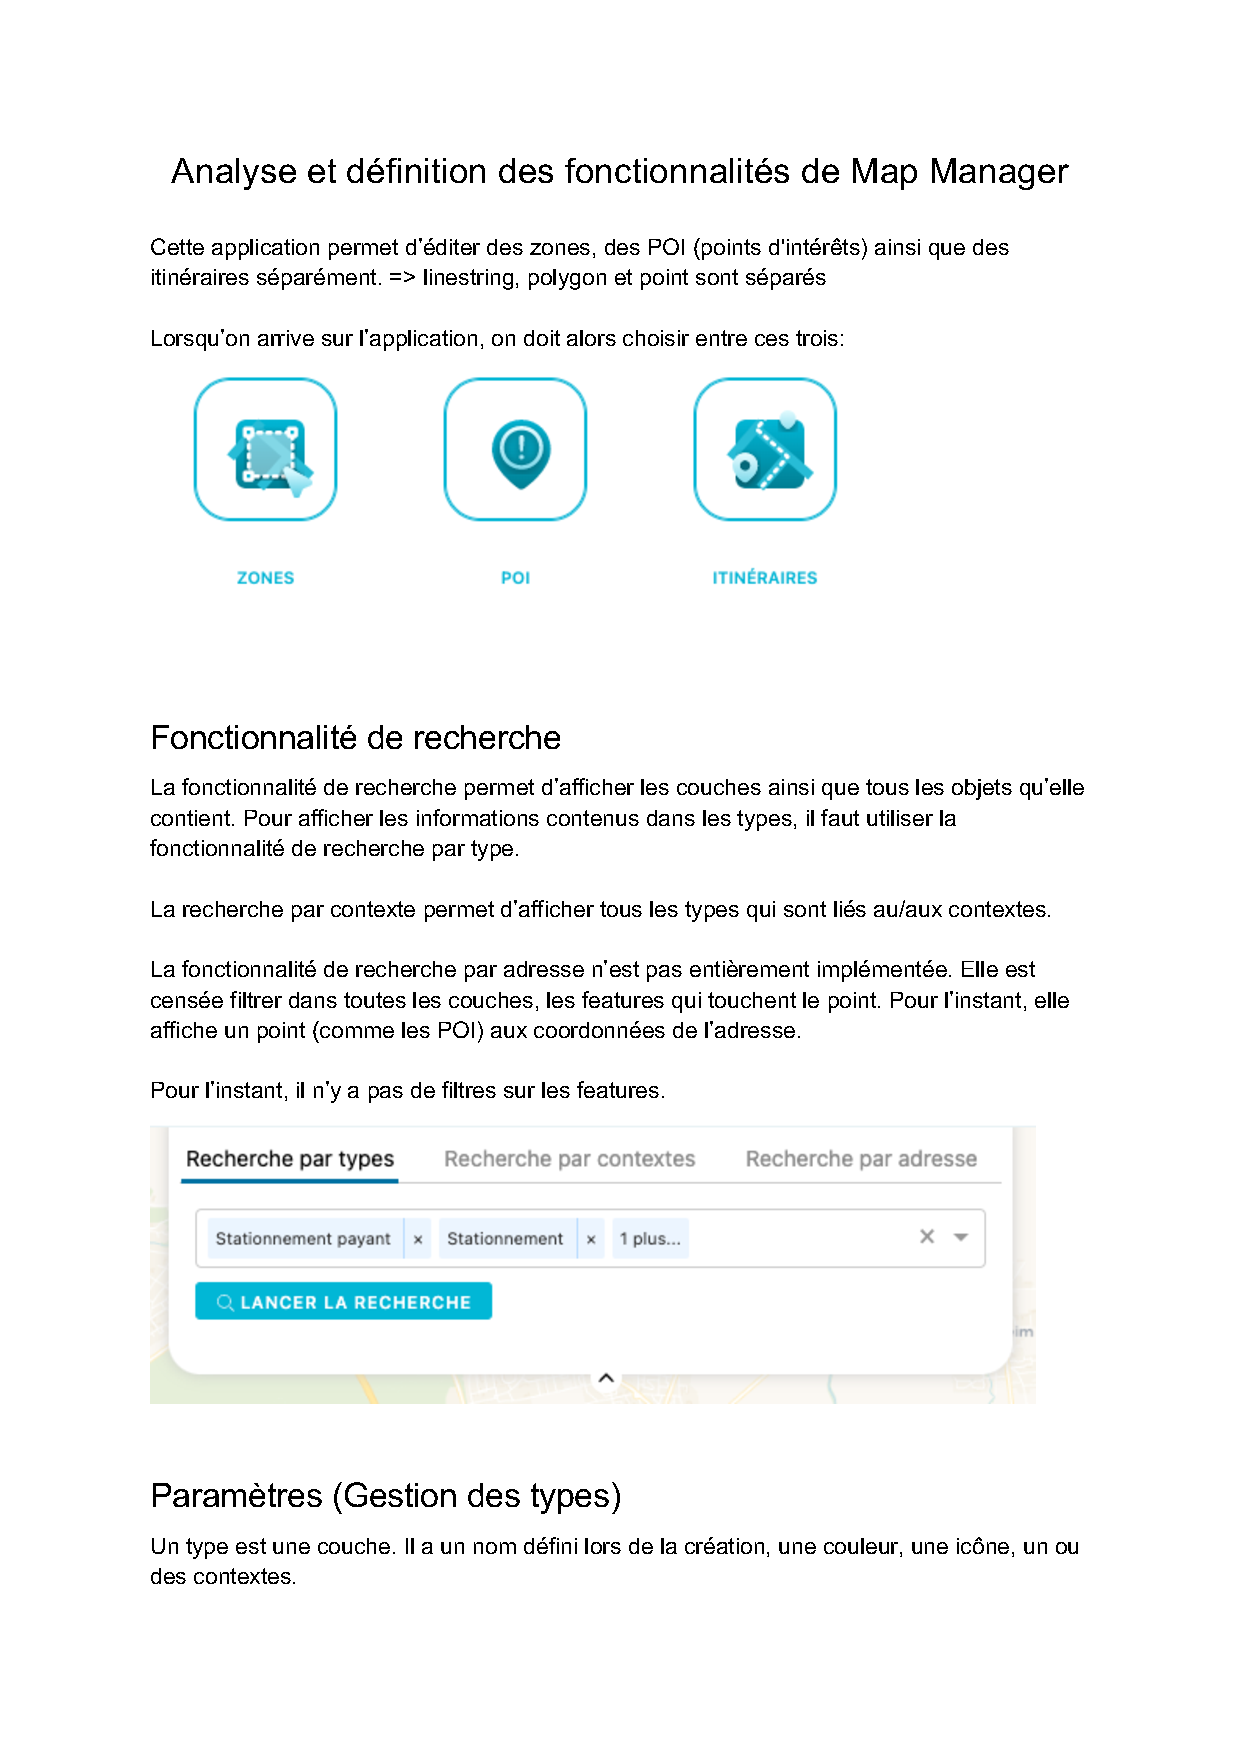
\includepdf[pages=1,pagecommand=\subsection*{\hypertarget{ANNEX2}{ANNEXE 2 – Document réalisé rendant compte des fonctionnalités de la version avant refonte}}, scale=0.8, offset=0 -1.5cm]{annex/analyse_fonctionnalites_existantes.pdf}
\includepdf[pages=2-, pagecommand={}, scale=0.8]{annex/analyse_fonctionnalites_existantes.pdf}
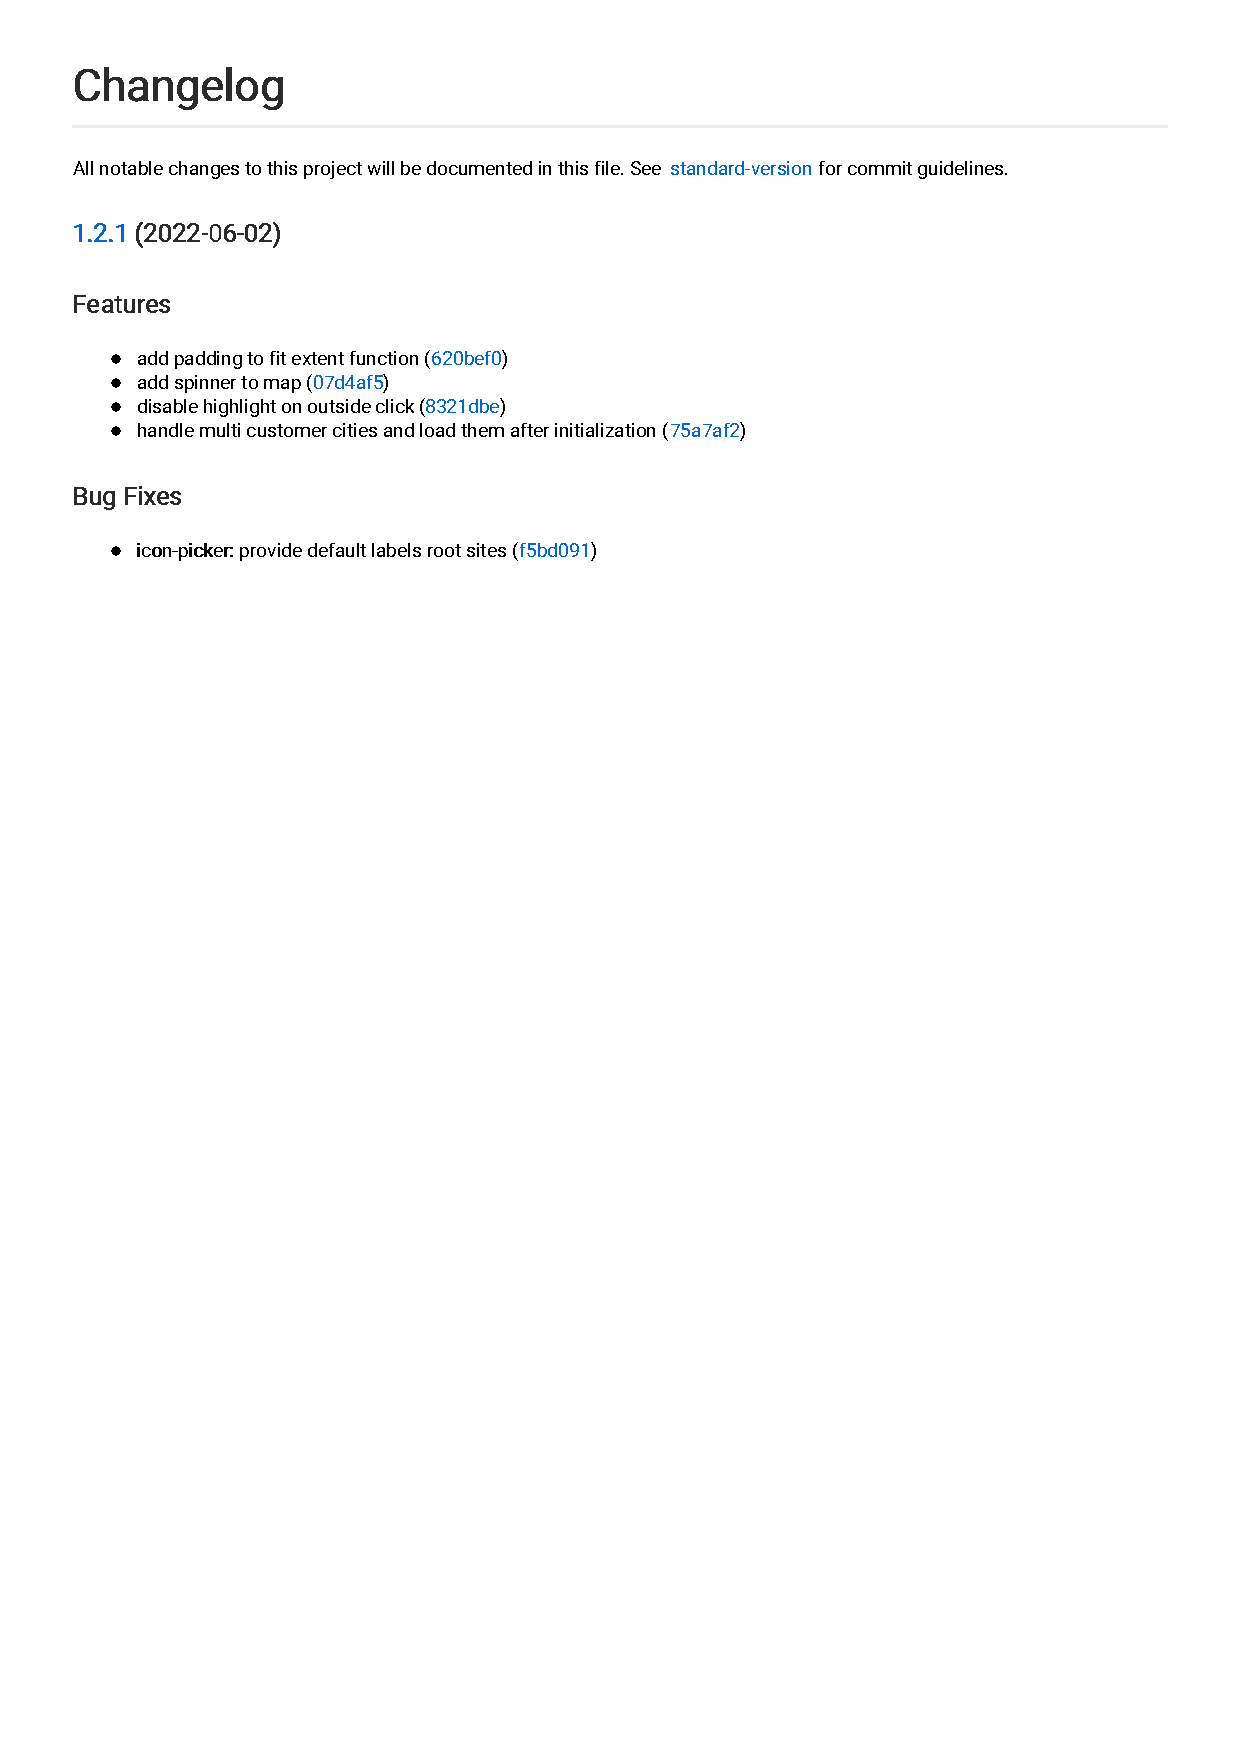
\includepdf[pages=1,pagecommand=\subsection*{\hypertarget{ANNEX1}{ANNEXE 3 – Changelog généré automatiquement pour la version 1.2.1}}, scale=0.8, offset=0 -2.5cm]{annex/CHANGELOG.pdf}

\end{document}